\documentclass[border=3]{standalone}
\usepackage{tikz}
\usepackage{tkz-euclide}

\begin{document}
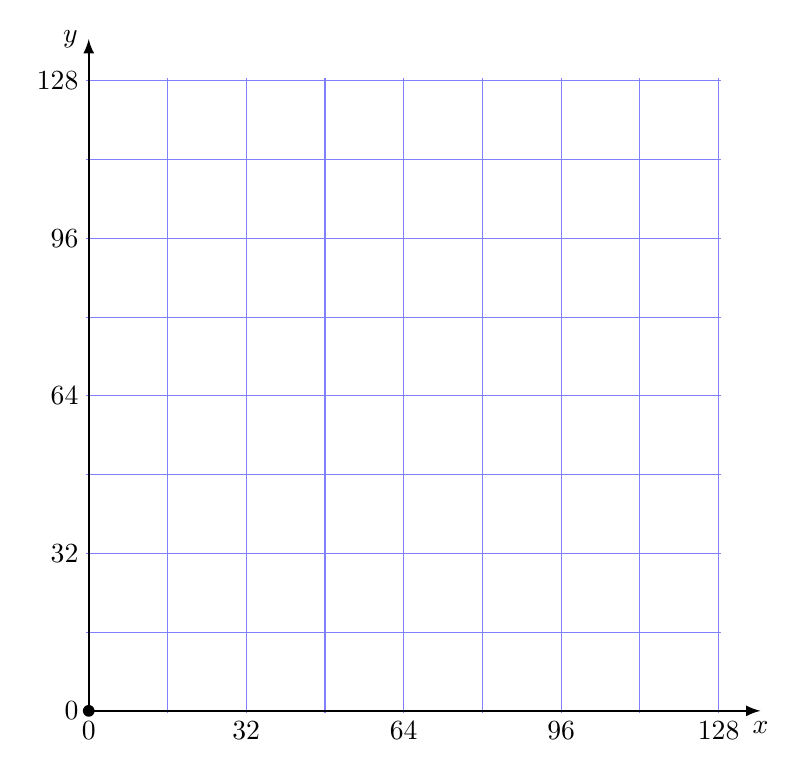
\begin{tikzpicture}
  \tkzInit[xmin=-0.5,xstep=16,xmax=128.5,
      ymin=-0.5,ystep=16,ymax=128.5]
  \tkzGrid[color=blue!50!white]
  \tkzDrawX[thick,>=latex,label=$x$]
  \tkzDrawY[thick,>=latex,label=$y$]

  \foreach \x in {0,32,64,96,128}
  { \tkzDefPoint(\x,0){$\x$}
    \tkzLabelPoints[below]($\x$) }

  \foreach \y in {0,32,64,96,128}
  { \tkzDefPoint(0,\y){$\y$}
    \tkzLabelPoints[left]($\y$) }

  \tkzDefPoint(0,0){O}
  %\tkzLabelPoint[](O){$(0,0)$}
  \node at (O)[circle,fill,inner sep=1.5pt]{};
\end{tikzpicture}
\end{document}
